%% Nivio: 22/jan/06 23/jan/06 29/jan
% Time-stamp: <Monday 30 Jan 2006 03:52:42am EDT yoshi@ime.usp.br>
\section{Introduction}
\label{sec:intro}

\enlargethispage{2\baselineskip}
Suppose~$U$ is a universe of \textit{keys} of size $u$.
Let $h:U\to M$ be a {\em hash function} that maps the keys from~$U$
to a given interval of integers $M=[0,m-1]=\{0,1,\dots,m-1\}$.
Let~$S\subseteq U$ be a set of~$n$ keys from~$U$, where $ n \ll u$.
Given a key~$x\in S$, the hash function~$h$ computes an integer in
$[0,m-1]$ for the storage or retrieval of~$x$ in a {\em hash table}.
% Hashing methods for {\em non-static sets} of keys can be used to construct
% data structures storing $S$ and supporting membership queries
% ``$x \in S$?'' in expected time $O(1)$.
% However, they involve a certain amount of wasted space owing to unused
% locations in the table and waisted time to resolve collisions when
% two keys are hashed to the same table location.
A perfect hash function maps a {\em static set} $S$ of $n$ keys from $U$ into a set of $m$ integer 
numbers without collisions, where $m$ is greater than or equal to $n$. 
If $m$ is equal to $n$, the function is called minimal. 

% Figure~\ref{fig:minimalperfecthash-ph-mph}(a) illustrates a perfect hash function and
% Figure~\ref{fig:minimalperfecthash-ph-mph}(b) illustrates a minimal perfect hash function (MPHF).
% 
% \begin{figure}
% \centering
% \scalebox{0.7}{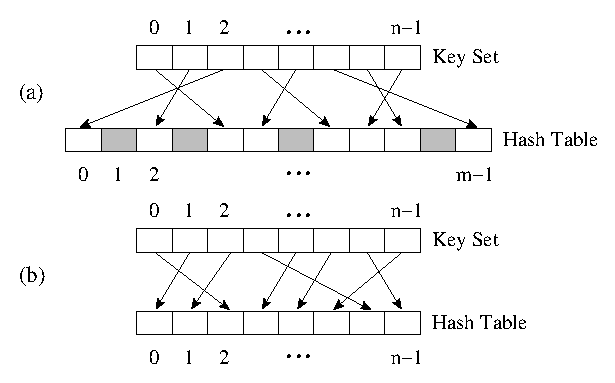
\epsfig{file=figs/minimalperfecthash-ph-mph.ps}}
% \caption{(a) Perfect hash function (b) Minimal perfect hash function (MPHF)}
% \label{fig:minimalperfecthash-ph-mph}
% %\vspace{-5mm}
% \end{figure}

Minimal perfect hash functions are widely used for memory efficient storage and fast 
retrieval of items from static sets, such as words in natural languages, 
reserved words in programming languages or interactive systems, universal resource 
locations (URLs) in web search engines, or item sets in data mining techniques. 
Search engines are nowadays indexing tens of billions of pages and algorithms
like PageRank~\cite{Brin1998}, which uses the web link structure to derive a
measure of popularity for Web pages, would benefit from a MPHF for storage and 
retrieval of such huge sets of URLs. 
For instance, the TodoBr\footnote{TodoBr ({\texttt www.todobr.com.br}) is a trademark of 
Akwan Information Technologies, which was acquired by Google Inc. in July 2005.}
search engine used the algorithm proposed hereinafter to 
improve and to scale its link analysis system. 
The WebGraph research group~\cite{bv04} would 
also benefit from a MPHF for sets in the order of billions of URLs to scale
and to improve the storange requirements of their algorithms on Graph compression. 

 Another interesting application for MPHFs is its use as an indexing structure 
 for databases. 
 The B+ tree is very popular as an indexing structure for dynamic applications 
 with frequent insertions and deletions of records. 
 However, for applications with sporadic modifications and a huge number of 
 queries the B+ tree is not the best option, 
 because it performs poorly with very large sets of keys 
 such as those required for the new frontiers of database applications~\cite{s05}.
 Therefore, there are applications for MPHFs in 
 information retrieval systems, database systems, language translation systems, 
 electronic commerce systems, compilers, operating systems, among others.

Until now, because of the limitations of current algorithms,
the use of MPHFs is restricted to scenarios where the set of keys being hashed is 
relatively small.
However, in many cases it is crucial to deal in an efficient way with very large
sets of keys. 
Due to the exponential growth of the Web, the work with huge collections is becoming
a daily task. 
For instance, the simple assignment of number identifiers to web pages of a collection 
can be a challenging task. 
While traditional databases simply cannot handle more traffic once the working 
set of URLs does not fit in main memory anymore~\cite{s05}, the algorithm we propose here to
construct MPHFs can easily scale to billions of entries.
% using stock hardware.

As there are many applications for MPHFs, it is 
important to design and implement space and time efficient algorithms for 
constructing such functions. 
The attractiveness of using MPHFs depends on the following issues:
\begin{enumerate}
\item The amount of CPU time required by the algorithms for constructing MPHFs.
\item The space requirements of the algorithms for constructing MPHFs.
\item The amount of CPU time required by a MPHF for each retrieval.
\item The space requirements of the description of the resulting MPHFs to be
  used at retrieval time.
\end{enumerate}

\enlargethispage{2\baselineskip}
This paper presents a novel external memory based algorithm for constructing MPHFs that 
is very efficient in these four requirements.
First, the algorithm is linear on the size of keys to construct a MPHF,
which is optimal.
For instance, for a collection of 1 billion URLs 
collected from the web, each one 64 characters long on average, the time to construct a
MPHF using a 2.4 gigahertz PC with 500 megabytes of available main memory
is approximately 3 hours.
Second, the algorithm needs a small a priori defined vector of $\lceil n/b \rceil$
one byte entries in main memory to construct a MPHF.
For the collection of 1 billion URLs and using $b=175$, the algorithm needs only
5.45 megabytes of internal memory.
Third, the evaluation of the MPHF for each retrieval requires three memory accesses and
the computation of three universal hash functions.
This is not optimal as any MPHF requires at least one memory access and the computation
of two universal hash functions.
Fourth, the description of a MPHF takes a constant number of bits for each key, which is optimal.
For the collection of 1 billion URLs, it needs 8.1 bits for each key,
while the theoretical lower bound is $1/\ln2 \approx 1.4427$ bits per 
key~\cite{m84}.

